\documentclass{article}
\usepackage{fancyhdr}
\usepackage[utf8]{inputenc}
\usepackage[english]{babel}
\usepackage{tikz, multicol, graphicx, etoolbox, enumerate, setspace, relsize, mathrsfs, verbatim}
\usepackage{amsmath, amsfonts, amssymb, amsthm, epsfig, epstopdf, titling, url, array, esvect, tikz-3dplot}
\usepackage{graphicx}
\usepackage{hyperref}

\usepackage{listings}
\usepackage{xcolor}

\definecolor{codegreen}{rgb}{0,0.6,0}
\definecolor{codegray}{rgb}{0.5,0.5,0.5}
\definecolor{codepurple}{rgb}{0.58,0,0.82}
\definecolor{backcolour}{rgb}{0.95,0.95,0.92}

\usepackage{pgfplots}
\usepackage{tcolorbox}
\usepackage{amsthm}
\usepackage{cancel}
\usepackage[left=1in,right=1in,top=1in,bottom=1in]{geometry}
\usepackage[tableaux]{prooftrees}

\lstdefinestyle{mystyle}{
    backgroundcolor=\color{backcolour},   
    commentstyle=\color{codegreen},
    keywordstyle=\color{magenta},
    numberstyle=\tiny\color{codegray},
    stringstyle=\color{codepurple},
    basicstyle=\ttfamily\footnotesize,
    breakatwhitespace=false,         
    breaklines=true,                 
    captionpos=b,                    
    keepspaces=true,                 
    numbers=left,                    
    numbersep=5pt,                  
    showspaces=false,                
    showstringspaces=false,
    showtabs=false,                  
    tabsize=2
}

\lstset{style=mystyle}

\pagestyle{fancy}
\fancyhf{}
\fancyhead[L,RO]{Tasksheet 7}
\fancyhead[R,RO]{Fundamentals of Computational Mathematics}
\fancyfoot[L,RO]{Xiang Gao}
\fancyfoot[R,RO]{Math 4610}
\renewcommand{\headrulewidth}{0.4pt}% Default \headrulewidth is 0.4pt
\renewcommand{\footrulewidth}{0.4pt}% Default \footrulewidth is 0pt
\def\checkmark{\tikz\fill[scale=0.4](0,.35) -- (.25,0) -- (1,.7) -- (.25,.15) -- cycle;} 

\begin{document}

\section*{Task 1}
I have created the following routine for generating an upper triangular matrix that satisfies the following definition for its entries:
$$a_{i, j} = \begin{cases} 0, & j < i \\ i + j - 1, & j \geqslant i\end{cases}$$
\lstinputlisting[language=Python]{matrixU.py}
The routine can also be found \href{https://github.com/GoByMark/math4610/blob/main/Homework_Tasks/Tasksheet_07/src/matrixU.py}{here}.\\
And I used the following code to find the solution to the upper triangular matrix $A$ that satisfies the following equation 
$$A x = b$$
where $A$ is created by user's choice, with $b_i = 1$. 
\lstinputlisting[language=Python]{Task_1.py}
The routine can also be found \href{https://github.com/GoByMark/math4610/blob/main/Homework_Tasks/Tasksheet_07/src/Task_1.py}{here}, with the following output:
\begin{center}
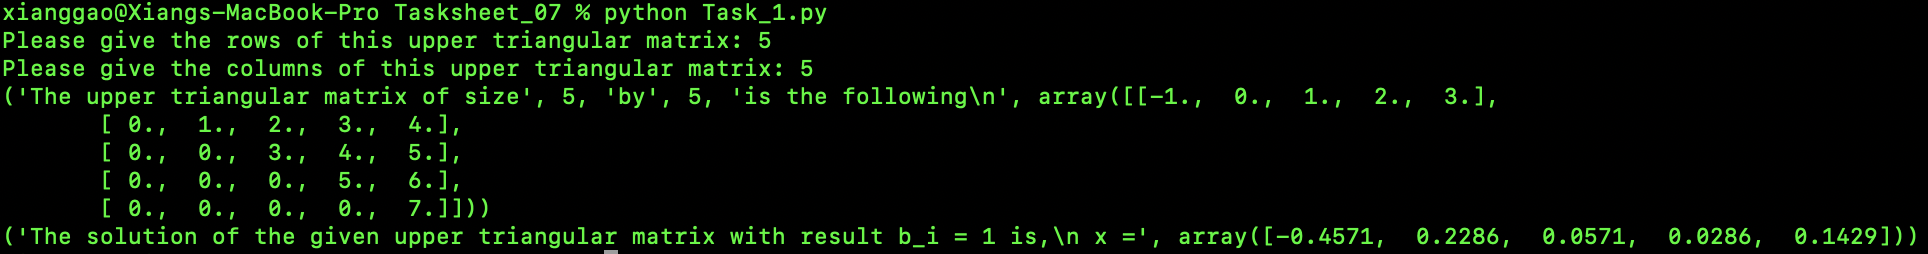
\includegraphics[width=\textwidth]{Screenshots/1.png}
{\bf Figure 1.} Running the Code From the Terminal.
\end{center}
\newpage
\raggedright However, since this looks a little bit ugly, I will from now on use the result from my IDE, which is the following
\begin{center}
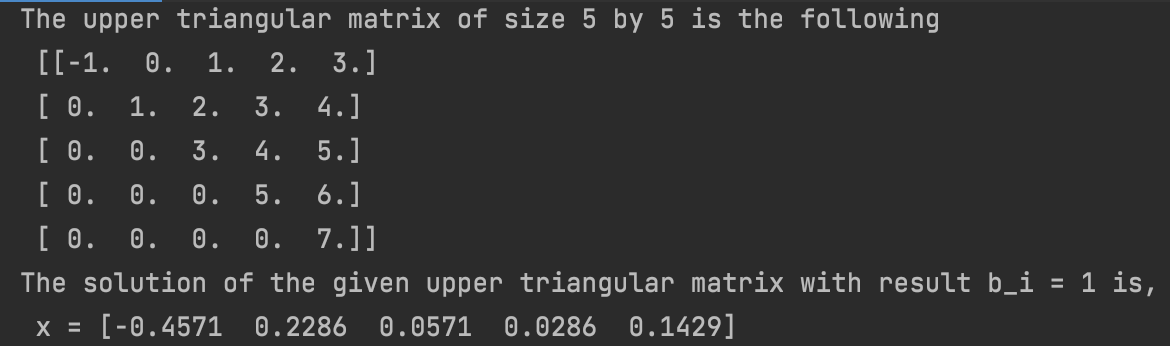
\includegraphics[width=\textwidth]{Screenshots/1better.png}
{\bf Figure 2.} Result of Task 1 from the IDE(PyCharm).
\end{center}

\section*{Task 2}
I have created the following routine for generating an lower triangular matrix, notice that there are two functions in this routine, I did this just to reminds myself of some linear algebra:
\lstinputlisting[language=Python]{matrixL.py}
The routine can also be found \href{https://github.com/GoByMark/math4610/blob/main/Homework_Tasks/Tasksheet_07/src/matrixL.py}{here}.\\
And I used the following code to find the solution to the lower triangular matrix $A$ that satisfies the following equation 
$$A x = b$$
where $A$ is created by user's choice, with $b_i = 1$. 
\lstinputlisting[language=Python]{Task_2.py}
The routine can also be found \href{https://github.com/GoByMark/math4610/blob/main/Homework_Tasks/Tasksheet_07/src/Task_2.py}{here}, with the following output:
\begin{center}
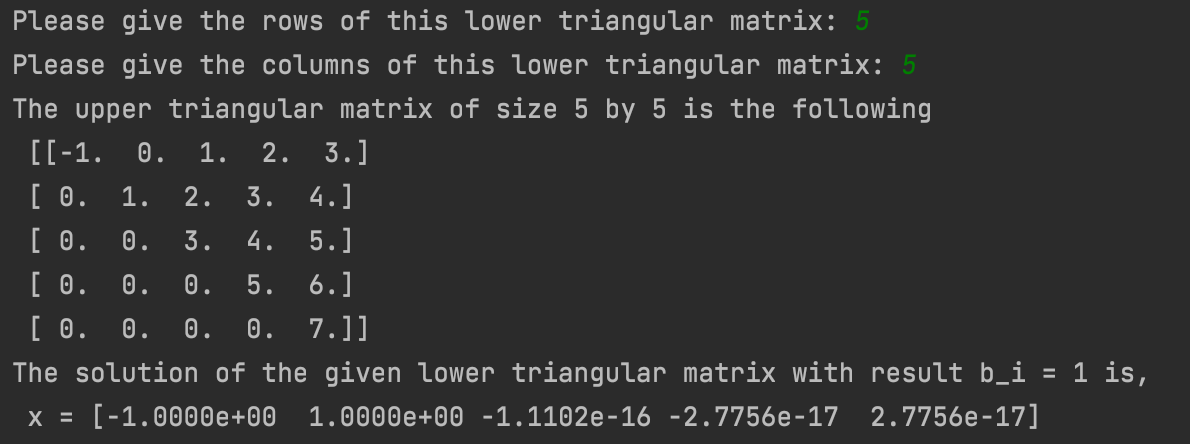
\includegraphics[width=\textwidth]{Screenshots/2.png}
{\bf Figure 3.} Result of Task 2 from the IDE(PyCharm).
\end{center}

\section*{Task 3}
This is the routine I've created for generating a $n \times n$ random square matrix. It can be found \href{https://github.com/GoByMark/math4610/blob/main/Homework_Tasks/Tasksheet_07/src/matrixS.py}{here}.
\lstinputlisting[language=Python]{matrixS.py}
This is the routine I've created for generating a $n \times n$ diagonal square matrix. It can be found \href{https://github.com/GoByMark/math4610/blob/main/Homework_Tasks/Tasksheet_07/src/matrixD.py}{here}.
\lstinputlisting[language=Python]{matrixD.py}

\section*{Task 4}
Use the previous routine, I've created the following code to solve the systems of equations as mentioned in {\bf Task 1} and {\bf Task 2}:
\lstinputlisting[language=Python]{Task_4.py}
The routine can also be found \href{https://github.com/GoByMark/math4610/blob/main/Homework_Tasks/Tasksheet_07/src/Task_4.py}{here}, with the following output:
\begin{center}
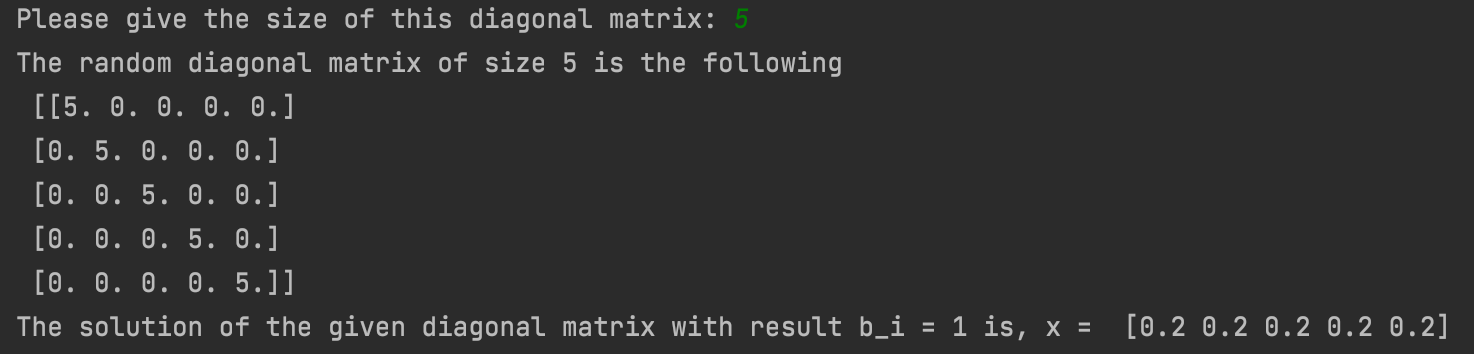
\includegraphics[width=\textwidth]{Screenshots/4.png}
{\bf Figure 4.} Result of Task 4 from the IDE(PyCharm).
\end{center}

\section*{Task 5}
I have written the following code to get the row-reduce-echelon form of any random square matrix generated by the routine mentioned in {\bf Task 4} with a given size $n \times n$:
\lstinputlisting[language=Python]{Task_5.py}
The routine can also be found \href{https://github.com/GoByMark/math4610/blob/main/Homework_Tasks/Tasksheet_07/src/Task_5.py}{here}, with the following output:
\begin{center}
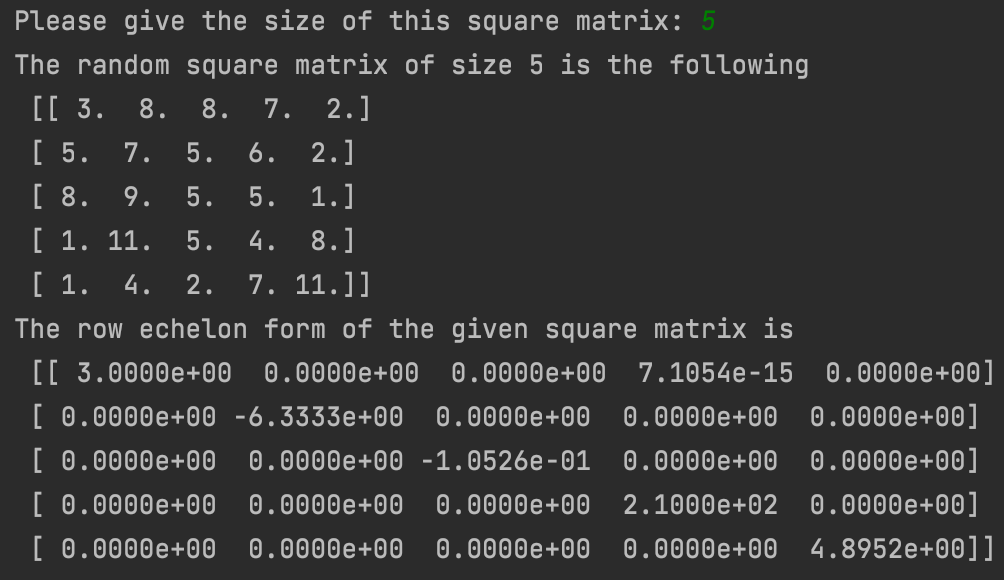
\includegraphics[width=\textwidth]{Screenshots/5.png}
{\bf Figure 5.} Result of Task 5 from the IDE(PyCharm).
\end{center}

\section*{Task 6}
From this \href{https://ocw.mit.edu/ans7870/2/2.086/F12/MIT2_086F12_notes_unit5.pdf}{online pdf}\footnote{https://ocw.mit.edu/ans7870/2/2.086/F12/MIT2086F12notesunit5.pdf} I found, when it comes to the conditions on matrices that ensure we will be able to compute the solution of a linear system of equations. The following has to be mentioned:
\begin{itemize}
\item The system has to be well-posed, that is: $n$ equations in $n$ unknowns;
\item The inverse of the matrix $K$, $K^{-1}$ must exist.
\end{itemize}
For the second item of the list, without the condition $K^{-1}$ exist, back substitution is required rather then just Gaussian elimination.
\end{document}